\documentclass[12pt,a4paper]{report}
\usepackage[utf8]{inputenc}
\usepackage[french]{babel}
\usepackage[T1]{fontenc}
\usepackage{amsmath}
\usepackage{amsfonts}
\usepackage{amssymb}
\usepackage{graphicx}
\author{Malo Kerebel}

\usepackage{hyperref}
\hypersetup{
    colorlinks,
    citecolor=black,
    filecolor=black,
    linkcolor=black, urlcolor=black
}
\usepackage{mathrsfs}

\usepackage{tikz}

%Macro
\newcommand{\ens}[1]{\mathbb{#1}}

\begin{document}


\begin{titlepage}

\centering{
	
	{\scshape\LARGE Université de Bretagne Occidentale \par}
	\vspace{1cm}
	{\scshape\Large Note de cours\par}
	\vspace{1.5cm}
	{\huge\bfseries Physique statistique\unskip\strut\par}
	\vspace{2cm}
	{\Large\itshape Malo Kerebel \par}
	
	\vfill

	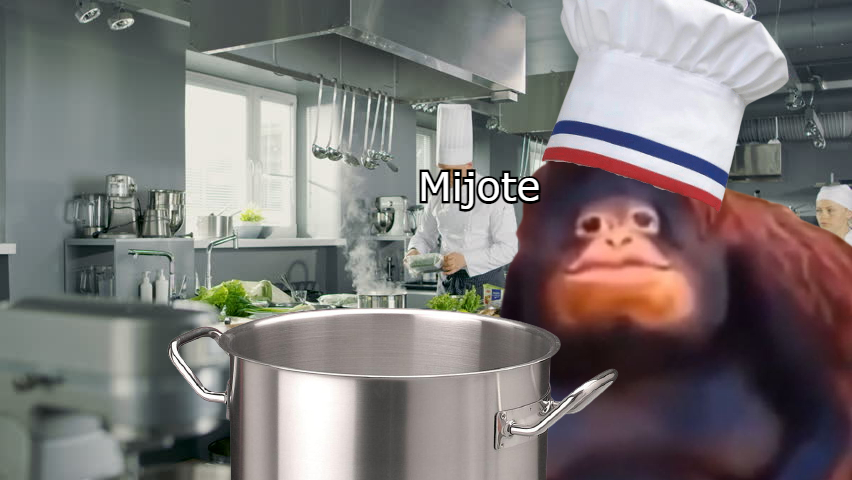
\includegraphics[scale=0.25]{monkey_mijote.jpg}	
	
	\vfill
	Cours par\par2
	Jean-Philippe \textsc{Jay}

	\vfill

% Bottom of the page
	{\large Semestre 6, année 2020-2021 \par}
}
\end{titlepage}

\tableofcontents

\chapter{Introduction générale}
\begin{center}
\textbf{CM1 (2021-01-12)}
\end{center}

physique statistique : étude du mouvement de gaz à l'échelle macroscopique.
Différences entre fermion et boson : leur spin, fermion spin demi entier (eg. les électrons), boson particule à spin entier (eg photon)\par
\quad \par
Bibliographie:
Physique Statistique, B. Diu, C. uthmann, D.Lederer\\
Physique Statistique, H. Ngp, C. Ngo\par
\quad \par

\section{Buts de la physique statistique}
Unifier le macroscopique et le microscopique, au $\text{XIV}^{\text{\`eme}}$ siècle, on a la thermodynamique, la mécanique et l'électro-magnétisme mais rien qui relie les uns aux autres.

Au niveau microscopique on a $\approx 10^{23}$ paramètres (de l'ordre du nombre d'Avogadro), auquel il faut avoir la vitesse et la position, il est impossible d'appliquer les résultats de la mécanique macroscopique dessus.
La physique statistique a donc pour but d'expliquer les comportements collectifs, de particules mais les résultats peuvent s'étendre à des réseaux de neurones ou des comportements de foules.

\section{Combinatoire}
Le dénombrement des objets ou des configurations. 2 systèmes indépendants A et B, ayant $\Omega_a$ et $\Omega_b$ configurations, il y a \(\Omega_a \times \Omega_b\) configurations possibles pour la juxtaposition de A et B.

\begin{center}
\textbf{CM2 (2021-01-14)}
\end{center}

Le nombre de permutations de N objets parmi N est N!

Le nombre de combinaisons sans répétitions s'obtient avec :
\[
	C^k_n = \dfrac{n!}{k!(n-k)!}
\]

\section{Probabilités - Statistiques}

événement aléatoire : résultat possible d'une expérience

Variable aléatoire : variable qui peut prendre l'une quelconque de ses valeurs possibles, inconnue d'avance. Discrète il y a un nombre finie de valeurs, continue il y a un nombre infini de valeurs possibles.

\paragraph{Propriétés}
\begin{enumerate}
	\item \(0 \leq P_m \leq 1 \quad \forall m\)
	\item \(\sum_m P_m = 1\) (normalisation)
\end{enumerate}

Pour une variable aléatoire continue on utilise la densité de probabilité, que la variable \(\in [x, x +\delta x]\)
\[
	w(x) = \lim_{\delta_x \rightarrow 0^+} \frac{\delta P(x)}{\delta_x}
\]
\[
	dP(x) = w(x)dx = \lim_{N \rightarrow \infty} \frac{dN(x)}{N}
\]
De même il y a la normalisation :
\[
	\int_{-\infty}^{+\infty} w(x)dx = 1
\]

Quand on est dans les bonne conditions :
\[
	P(e_1 ou e_2) = P(e_1) + P(e_2)
\]
\[
	P(e_1 et e_2) = P(e_1)\cdot P(e_2)
\]

L'écart quadratique moyen, ou variance, caratérise la dispersion de la distribution statistique, il est défini par :
\[
	(\Delta_f)^2 = \overline{(f - \overline{f})^2} = \overline{f^2} - (\overline{f})^2
\]
De même on définit l'écart-type \(\sigma\) comme la racine carrée de la variance :
\[
	\sigma = \sqrt{(\Delta_f)^2} = \Delta_f
\]

La moyenne de résultat est :
\[
	\overline{n} = pN
\]

\begin{center}
\textbf{CM3 (2021-01-19)}
\end{center}

Après calculs : \(\overline{n^2} = pN + p^2N(N-1)\)
Donc \(\sigma^2 = \overline{n^2} - (\overline{n})^2 = pN + p^2N^2 - p^N - p^2N^2 = pN - p^2N\)
\[
	\sigma^2 = N p q = Np(1-p)
\]

Ainsi on voit que l'écart type croit avec N :
(Cependant, la dispersion relative à la moyenne décroit)
\[
	\dfrac{\sigma}{\overline{n}} \sim \dfrac{\sqrt{N}}{N} = \dfrac{1}{\sqrt{N}}
\]

\subsection{Loi de Poisson}

Hypothèses :
\begin{itemize}
	\item[•] \(p \rightarrow 0\)
	\item[•] \(N \rightarrow +\infty\)
	\item[•] MAIS \(pN = \lambda\) reste une valeur finie.
\end{itemize}

La loi de poisson dit donc que la loi binomiale devient :
\[
	P(N, n) = \dfrac{\lambda^n}{n!}e^{-\lambda}
\]
La proba ne dépend pas du nombre d'expériences N
Exercice : Vérifier que c'est bien normalisé.
\[
	\sum_n P(N,n) = 1 = \sum_n \dfrac{\lambda^n}{n!}e^{-\lambda} = e^\lambda e^{-\lambda} = 1
\]

On a :
\[
	\overline{n} = \sigma^2 = \lambda
\]
On peut donc aussi écrire la loi de poisson sous la forme :
\[
	P = \dfrac{\overline{n}^n}{n!}e^{-\overline{n}}
\]

\subsection{Loi Gaussienne ou loi normale}

La densité de probabilité est :
\[
	w_G (c) = \dfrac{1}{\sqrt{2\pi \sigma^2}} e^{\left[ \dfrac{- (x-x_0)^2}{2\sigma^2} \right]}
\]
\(w_G\) dépend de 2 paramètres, le centre (ou la moyenne) \(x_0\) et la largeur \(\sigma\)

\subsection{Théorème de la limite centrale}

La distribution de la somme de N variables aléatoires indépendantes et de même loi devient gaussienne lorsque N devient grand

En particulier la loi binomiale \(\rightarrow\) loi gaussienne

Théorème important en physique stats, car les systèmes macroscopiques sont souvent constitué d'un très grand nombre d'éléments faiblement couplés.

Les variables libres de fluctuer ont alors une distribution gaussienne.

\section{Entropie statistique}

Les informations concernant le système physique sont incomplète.
L'entropie statistique mesure le manque d'information.

\subsection{Définition de l'entropie statistique}

Ensemble fini d'événements \(e_m (m = 1,2, \cdots , M)\) de proba \(P_m\).
Tout autre distribution implique un manque d'information

\textbf{Entropie statistique} :
\[
	S(P_1, P_2, \cdots, P_M) = -k \sum_{m=1}^M P_m \ln(P_m)
\]
Avec \(P_m \ln(P_m) = 0\) si \(P_m = 0\) et \(k = k_B = 1,380649 \times 10^{-23} J\cdot K^{-1}\) la constante de Boltzmann, seule l'ordre de grandeur et l'unité sont à retenir.

L'entropie est nulle si une des probabilités des événements possibles est de 1. Inversement l'entropie est maximale quand tous les événements sont équiprobables. L'entropie augmente avec le nombre d'événements possibles.

\section{Quelques résultat de maths}

\subsection{Approximation de Stirling}

Approximation utile pour plus tard :
Pour \(N \gg 1\), on a :
\[
	\ln(N!) \sim N \ln(N) - N
\]

\subsection{Intégrales gaussiennes}

\[
	\int_{-\infty}^{+\infty} e^{-\alpha x^2}dx = \sqrt{\dfrac{\pi}{\alpha}}
\]

\subsection{Méthode des multiplicateurs de Lagrange}

f fonction de n variables indépendantes. Il y a un maxima si :
\[
	\dfrac{\partial f}{\partial x_1} = \cdots = \dfrac{\partial f}{\partial x_n} = 0
\]

Si il y a une contraintes entre les variables, ex \(g(x_1, \cdots, x_n = 0\)
Pour prendre en compte cette contrainte, on introduit une nouvelle fonction, \(F = f \pm \lambda g\), \(\lambda\) paramètre de Lagrange.

\(dF = 0 \Rightarrow \dfrac{\partial f}{\partial x_j} \pm \lambda \dfrac{\partial g}{\partial x_j}\) avec \(j = 1, \cdots, n\)

\subsection{Volume sphère de dimension n - Fonction \(\Gamma\)}

Le volume d'une hypersphère dans un espace à n dimensions est :
\[
	V_n = C_n r^n \text{ avec } C_n = \dfrac{\pi^{n/2}}{\Gamma\left( \frac{n}{2} + 1 \right)}
\]

La fonction \(\Gamma\) est telle que :
\begin{align*}
	\Gamma(x) &= \int_0^{+\infty} e^{-t} t^{x - 1} dt\\
	\Gamma (x+1) &= x \Gamma(x)\\
	\Gamma (\frac{1}{2}) &= \sqrt{\pi}\\
	\Gamma (1) &= 1	
\end{align*}
Si \(n \in N\) on a :
\[
\Gamma (n + 1) = n!
\]	


\chapter{Description statistique d'un système physique}

\begin{center}
\textbf{CM4 (2021-01-26)}
\end{center}

\section{Description quantique}

Un état quantique est défini par un ket : \(\vert \varphi \rangle\)
Son évolution est donnée par l'équation de Schrödinger :
\[
	i\hbar \dfrac{\partial \vert \varphi \rangle}{\partial t} = \hat{H} \vert \varphi \rangle
\]

Avec H l'hamiltonien du système (opérateur associé à l'énergie)
\[
	\hat{H} = \hat{T} + \hat{V} = \dfrac{\hat{P}}{2m} + \hat{V}
\]

Si \(\hat{H}\) est indépendant du temps on a alors un système conservatif. les valeur propres de \(\hat{H}\)H donnes les valeurs possibles de l'énergie.

En général, les énergies sont dégénérées : plusieurs états peuvent avoir la même énergie.

Pour un état quantique macroscopique, on a un mélange statistique des états purs.
On a donc la valeur moyenne dans l'état pur \(\vert \varphi \rangle\) : \(\langle A_m \rangle = \langle \varphi_m \vert \hat{A} \vert \varphi_m \rangle\)

On aura à calculer des sommes sur les états stationnaires (\(\ell\)) de la forme :
\[
	\overline{A} = \sum_{(\ell)} P_{\ell} A_{\ell}
\]

Il ne faut pas confondre les niveaux d'énergie et les états stationnaires, en général, plusieurs états microscopisques (\(\ell\)) distincts correspondent à la même énergie

Mais la quantité à sommmer peut ne dépendre que de l'énergie \(E_\ell\) de l'état (\(\ell\))

On peut remplacer \(\sum_{\text{état(}\ell)}\) par \(\sum_{\text{Niveau d'énergie}}\)

Pour un système macroscopique, l'écart entre 2 niveaux consécutifs d'énergie est très faible et on peut l'approximer comme continu pour pouvoir intégrer plutôt que faire la somme discrète.

On définit la densité d'états \(dn(E)\) nombre d'état dont l'énergie est comprise entre E et E + dE.
On peut faire :
\[
	\overline{A} = \sum_{E_\ell} g(E_\ell)f(E_\ell) = \int_{E_0}^{\infty} \rho(E)f(E) dE
\]

Cette approximation n'est plus bonne si f(E) varie très brusquement.

En pratique il est plus facile de calculer le nombre d'état ne dépassant pas une certaine énergie \(\Phi(E)\), on a donc \(dn(E) = \Phi(E+dE) - \Phi(E)\) d'où comme \(dE \rightarrow 0\) : 
\[
	\rho(E) = \dfrac{d\Phi}{dE}
\]

\subsection{N particules dans une boite de volume V-Gaz parfait}

N particules sans interaction dans une boite de volume \( V \equiv GP\)

Énergies totale :
\[
	E = \sum_{i = 1}^N \varepsilon_i = (n_{x1}^2 + n_{y1}^2 + n_{z1}^2 + \cdots n_{xN}^2 + n_{yN}^2 + n_{zN}^2)\varepsilon_0
\]

Donc le nombre d'état à  une énergie inférieure à E est :
\[
	\Phi(E) = \dfrac{1}{2^{3N}} \dfrac{\pi^{3N/2}}{\Gamma(3N/2 + 1)} \left( \dfrac{E}{\varepsilon_0}\right)^{3N/2}
\]

La densité d'état est donc :
\[
	\rho(E) \propto E^{\frac{3N}{2} - 1}
\]

\subsection{Particules discernables - indiscernables}

En physique classique les particules sont discernables car on peut suivre les trajectoires de chacune d'entre elles.
En quantique, la notion de trajectoire n'existe pas.
Il est donc impossible de distingur deux quantons identiques indépendants, ils sont indiscernables.
En fais ce sont les positions occupées par les quantons qui seront discernables, ou pas.

La fonction d'onde d'un système de particules identiques est symétrique ou antisymétrique par rapport à leur permutation

Si la fonction d'onde est symétrique on a des bosons.
Les bosons ont donc un spin entier : \(s = n \hbar \quad  n \in \ens{N}\)

Si la fonction est antisymétrique, on a des fermions, avec un spin demi-entier \(s = (n + \frac{1}{2}) \hbar \quad n \in \ens{N}\)

\begin{center}
\textbf{CM5 (2021-02-02)}
\end{center}

\section{Cas de particules discernables}

On a au total N particules et $n_r$ particules à un niveau d'énergie $\epsilon_r$ dégénéré $g_r$ fois.
Pour le $1^{\text{er}}$ niveau d'énergie on a $C_N^{n_1}$ façons de choisir $n_1$ particules parmi N.
Comme on a $g_1$ état de même énergie, il y a $g_1^{n_1}$ choix
\[
	\Omega_1 = C_N^{n_1} g_1^{n_1}
\]
Pour le $2^{\text{ème}}$ niveau, il ne reste que $N - n_1$ particules, on choisit $n_2$ parmi ces $N - n_1 \Rightarrow C_{N-n_1}^{n_2}$ choix possibles, il y a $g_2$ états $\Rightarrow g_2^{n_2}$.
etc... pour la suite :
\begin{align*}
	\Omega &= \prod_{i=1} \Omega_i\\
	&= \prod_{i=1} C_{N-\sum_{j=1}^{i-1} n_j}^{n_i} g_i^{n_i}\\
	&= \dfrac{N!}{n_1!(N-n_1)!} \times \dfrac{(N-n_1)!}{n_2!(N-n_1-n_2)!}\cdots \times g_1^{n_1} \cdot\\
	&= \dfrac{N!}{n_1!n_2! \cdots} g_1^{n_1}g_2^{n_2} \cdots\\
	&= N! \prod \dfrac{g_r^{n_r}}{n_r!}
\end{align*}


\subsection{Cas des fermions}

\subsection{Cas des bosons}

Un système est dilué si le nombre de particules $n_r$ à répartir dans les $g_r$ états est petit ($n_r \ll g_r$) alors on montre que :
\[
	\Omega^B \simeq \Omega^F \simeq \dfrac{1}{N!}\Omega^{\text{Discernable}}
\]

$\Rightarrow$ Bosons et fermions dilués quasi équivalents aux particules classiques mais avec un facteur d'indiscernabilité : $\frac{1}{N!}$

\section{Description d'un système classique}

\begin{center}
\textbf{CM5 (2021-02-08)}
\end{center}

\subsection{État microscopique - description classique}

La description quantique n'est pas toujours nécessaire. Le système est décrit par les positions et les impulsions des particules du système. Les lois de Newton décrivent les évolutions du système.

États du système est décrit par l'espace des phases, de dimension 6N, avec N le nombre de particules. La position en \(x\), \(y\) et \(z\) et l'impulsion en $p_x$, $p_y$ et $p_z$.
En mécanique classique le nombre d'état est infini (l'énergie n'est pas multiple entière d'un quantum d'énergie), les variables sont donc continues.

On quadrille l'espace en case de largeur $\delta_p$ et $\delta_q$, le volume d'une case est donc de \(h_0 = \delta_p \delta_q\) et son unité est le produit d'une longueur et d'une impulsion, son unité est donc des $J\cdot s$ (équivalent à l'unité de \(\hbar\)).

Plus on prend une cellule petite, plus la précision est élevée. classiquement \(h_0\) peut-être aussi petit que l'on veut, mais la physique quantique impose \(h_0 \geq h\), la constante de Planck.

Si le nombre de paramètres nécessaire est grand, on utilise les probabilité pour définir un état macroscopique.
L'état macroscopique est donc caractérisé par une densité de probabilité dans l'espace des phases.
\(dP = w\left( q, p; t\right) dq~dp\) :Probabilité que le système se trouve dans l'état {q, p} à \(dq~dp\) près.

La valeur moyenne d'une grandeur physique f :
\[
	\overline{f} = \int f(q,p; t) w(q,p;t)dq dp
\]

L'approche classique est valable si l'action caractéristique du système est très supérieure à \(\hbar\) avec :\\
(action) \(\equiv\) (Énergie) \(\times\) (temps) ou (Longueur) \(\times\) (quantité de mouvement)

Pour un gaz parfait, on a la vitesse moyenne :
\[
	\overline{v} = \sqrt{\dfrac{3 k_B T}{m}}
\]

Avec, \(\ell\) la distance moyenne entre les particule :\(\ell = \left( \frac{V}{N}\right)^{1/3}\)

et, \(\lambda\) la longueur d'onde thermique de De Broglie : \(\lambda = \frac{\hbar}{\sqrt{3mk_BT}}\)

L'approche classique est valide si \(\ell \gg \lambda\), soit lorsque la température est élevé et/ou lorsque la densité est faible.

Si on impose des contraites au système, le volume accessible de l'espace des phases est limité à \(\mathscr{V}_\phi\)
Alors le nombre de micro-états accessible au système est :
\[
	\dfrac{\mathscr{V}_\phi}{h_0^n} \text{ avec } h_0 = h
\]

\paragraph{Exemple} Une particule m dans une boite de volume V


\(E = \left( p_x^2 + p_y^2 + p_z^2\right)/2m\)

\(\Phi(E)\) est le nombre d'états dont l'énergie est inférieure à E :\\
\(p_x^2 + p_y^2 + p_z^2 \leq 2mE\)
\[
	\Phi(E) = \dfrac{V \frac{4}{3} \pi (2mE)^{3/2}}{h^3}
\]

\chapter{Ensemble microcanonique}

\section{Équilibre}

Au niveau microscopique on a toujours des fluctuations, même à l'équilibre.

\paragraph{Définition} Ensemble statistique

Collection d'un grand nombre de système identique (réplique du système initial)

\paragraph{Définition} Moyenne d'ensemble

La moyenne d'ensemble d'une grandeur A est :
\[
	\overline{A} = \sum_{(\ell)} P_\ell A_\ell
\]

Tous les ensembles sont pris au même instant, mais en pratique on ne peut prendre qu'un seul système.

\paragraph{Définition} Principe ergotique

On postule que dans un système à l'équilibre, la moyenne d'ensemble est :
\[
	\overline{A} = \sum_{(\ell)} P_\ell A_\ell = \underset{\tau \rightarrow \infty}{\lim} \dfrac{1}{\tau} \int_0^\tau A(t) dt = \langle A \rangle
\]

Principe essentiel en pratique : On mesure des moyennes temporelles mais la théorie est basée sur des moyennes d'ensemble.

\paragraph{Définition} Paramètres extérieurs

Propriétés fixées par des contraintes extérieures, valeurs statistiquement certaines même si il y a une incertitude expérimentale.

\paragraph{Définition} Variables internes

Propriétés libres de fluctuer au gré de l'agitation microscopique.

Selon les cas, une même grandeur peut être un paramètre extérieur ou une variable interne.

\paragraph{Définition} États accessibles

États microscopique vérifiant les contraintes extérieures, c'est-à-dire compatible avec les valeurs des paramètres extérieurs.

\paragraph{Postulat}

Pour un système isolé à l'équilibre macroscopique, tous les états accessibles ont la même probabilité.

Soit E l'énergie du système (fixée) et \(\delta E\) l'incertitude macroscopique associée.

Les états microscopique accessibles (\(\ell\)) sont ceux qui vérifient toutes les autres contraintes extérieures.

L'ensemble constitué de systèmes isolés identiques est appelé ensemble microcanonique. Dans cet ensemble seuls apparaissent les états (\(\ell\)) accessibles et ils apparaissent avec la même fréquence dans la limite \(\mathcal{N} \rightarrow \infty\), postulat fondamental \(\equiv\) principe du "désordre maximum" :

La distribution microcanonique est celle qui maximise l'entropie statistique (On parle de désordre mais ça représente plutot le manque d'information).

On associe une entropie appelée entropie microcanonique à la distribution microcanonique

\paragraph{Définition} Entropie microcanonique :

Les micro-états étant équiprobables, l'entropie microcanonique est :
\[
	S^* = k_B \ln \Omega
\]
Avec \(\Omega\) le nombre d'états accessibles.

\(\Omega(E,x, \delta	E )= \rho(E, x)\delta E \)

\(\ln \Omega = \ln \rho(E,x) + \ln \delta E\)

\(S^* (E,x) = k_B \ln \rho(E,x)\) et aussi \(S^* (E,x) = k_B \ln \Phi(E)\)

\begin{center}
\textbf{CM6 (2021-02-09)}
\end{center}

L'entropie \(S^\star\) est une valeur extensive

\paragraph{Temperature \(T^\star\)}

Définie par 
\[
	\dfrac{1}{T^\star} = \left( \dfrac{\partial S^\star}{\partial E}\right)_{V,N}
\]

\paragraph{Pression \(P^\star\)}

Définie par
\[
	\dfrac{p^\star}{T^\star} = \left( \dfrac{\partial S^\star}{\partial V}\right)_{E,N}
\]

\paragraph{Potentiel chimique \(\mu^\star\)}

Définie par
\[
	\dfrac{\mu^\star}{T^\star} = \left( \dfrac{\partial S^\star}{\partial N}\right)_{E,V}
\]

On a donc :
\[
	dS^\star = \dfrac{dE}{T^\star} + \dfrac{p^\star}{t^\star}dV + \dfrac{\mu^\star}{T^\star}dN
\]

On s'intéresse aux changements d'états d'équilibre d'un système isolé.

On prend un gaz isolé dans un volume V, on ouvre une enceinte vide de volume \(\Delta V\), plus d'états sont possibles, et donc l'entropie va augmenter.

La modification de contrainte extérieures augmente l'entropie et le prochain état d'équilibre correspond au nouveau maximum de son entropie.

\paragraph{Exemple}

Volume séparé en deux parties séparé par une paroi isolante qui devient diatherme. À l'équilibre final on aura l'état à l'entropie maximal, une température égal dans les deux parties du volume.

L'énergie du système est de \(E = E_1 + E_2\)

Initialement \(E_1\) et \(E_2\) sont des paramètres extérieurs mais après changement de la paroi, \(E_1\) et \(E_2\) deviennent des variables internes

\[
	w(E_1) = \dfrac{\omega(E,V,N,E_1)\delta E_1}{\Omega(E,V,N)}
\]
Avec \(\omega(E,V,N,E_1)\), le nombre d'états accessible au systeme tels que l'énergie de la zone 1 soit égale à \(E_1\) (à \(\delta E_1\) près) et \(\Omega(E,V,N)\) le nombre d'états accessibles.

À l'équilibre \(\tilde{E_1}\) maximise \(s^\star(E_1) = S_1^\star(E_1) + S_2^\star(E-E_1)\)

\[
	\dfrac{\partial s^\star}{\partial E_1}(E_1 = \tilde{E_1} = 0 = \dfrac{\partial S_1^\star}{\partial E_1} + \dfrac{\partial S_2^\star}{\partial E_2} \dfrac{\partial E_2}{\partial E_1}
\]
On a \(E_2 = E-E_1\), donc :
\[
	\dfrac{\partial E_2}{\partial E_1} = -1 \text{ et } \dfrac{\partial S_1^\star}{\partial E_1} (E_1 = \tilde{E_1}) - \dfrac{\partial S_2^\star}{\partial E_2} (E_2 = E - \tilde{E_1}) = 0
\]
\[
	\Leftrightarrow \dfrac{1}{T_1^\star} = \dfrac{1}{T_2^\star}
\]
\[
	\Leftrightarrow T_1^\star = T_2^\star
\]

\begin{center}
\textbf{CM7 (2021-02-16)}
\end{center}

QCM du début de scéance (J'ai pas eu le temps de corriger les questions avant la 11)

\paragraph{question 11}

P face 5 fois d'affilé :

1/32

\paragraph{question 12}

proba de 3 face sur 5 lancé:

\[
	P = C^5_3 * 0.5^5 = 5/16
\]

\paragraph{question 13}

9 plaques de 1 à 9 combien de nombre impaire de 3 chiffres différents :

On prend le nombre en décimale abc, pour que le nombre soit impaire, c = 1, 3, 5, 7 ou 9. Pour b, on a plus que 8 choix, et pour a plus que 7 choix. Le nombre totale :
\[
	5 \times 8 \times 7 = 280
\]

\paragraph{Question 14}

Une voiture de 3 place, combien de façon d'installer 6 personne dont seuleument 2 ont le permis. Le conducteur on a deux choix, pour le passager avant on a 5 choix, pour le passager arrière on a 4 choix:
\[
	= 2 \times 5 \times 4 = 40
\]

\paragraph{Question 15}

Installer 3 filles et 3 garçon sur un banc, on a 
\[
	3! \times 2! \times 2 = 72 
\]

\paragraph{Question 16}

Loi binomiale :
\[
	P(N, n) = \dfrac{N!}{n!(N-n)!} p^n \times q^{N-n}
\]

\paragraph{Question 17}

Moyenne de la loi binomiale : \(pN\)

\paragraph{Question 18}

Distribution Gausienne :
\[
	\omega_G(x) = \dfrac{1}{\sqrt{2\pi \sigma^2}} e^{-\dfrac{(x - x_0)^2}{2\sigma^2}}
\]

\paragraph{Question 19}

L'écart type le plus grand est quand la fonction est aplatie donc courbe bleu foncé

\paragraph{Question 20}

L'entropie statistique mesure le manque d'information sur le système

\paragraph{Question 21}

L'entropie statistique est :
\[
	S(P_1, P_2, \cdots, P_M) = -k \sum_{m=1}^M P_m \ln(P_m)
\]

\paragraph{Question 22}

L'entropie statistique ne peut pas être négative (car la constante de Boltzmann n'est pas négative)

\paragraph{Question 23}

L'entropie statistique est maximale lorsque tous les évenements ont la même probabilité de se produire

\paragraph{Question 24}

Une approximation de \(\ln(N!)\) est :
\[
	\ln(N!) = N \ln(N) - N
\]

Retour au cours :

\[
	T_1^\star = T_2^\star
\]
\[
	\dfrac{1}{C_{V_1}} + \dfrac{1}{C_{V_2}} > 0
\]


Si \(C_{V_1} \gg C_{V_2}\) (La capacité calorifique à volume constant)
\subsubsection{Conséquence}
	La capacité calorifique est positive à l'équilibre \(\Leftrightarrow T^\star\) d'un système est 	fonction croissante de son énergie.

	\((\Delta E_1)^2 = \sigma^2_{E_1} = kT^2 C_{V_1}\)
	\(\Rightarrow\) la capacité calorifique reflète les fluctuations de \(E_1\), c'est le théorème de 	fluctuation dissipation

\begin{align*}
	&T_1^\star (E_1) \nearrow \text{ Est croissante en focntion de } E_1\\
	&T_2^\star (E_2) \nearrow \text{ mais } T_2^\star (E_1) \searrow\\
\end{align*}

La chaleur passe du système de température microcanonique la plus élévé à celui de température plus basse

Ça implique le deuxième principe de la thermodynamique.
\subsubsection{deuxième principe de la thermodynamique}

	La chaleur s'écoule du corps le plus "chaud" vers celui le plus "froid"

\quad \\ %C'est moche de faire ça mais ça rend plus joli rapidement
La temérature microcanonique \(T^\star\) a donc les caractéristiques habituelles d'une température.

\paragraph{Remarque} Si \(C_V\) indépendate de la température

\[
	E_1 + E_2 = E \Rightarrow C_{V_1} T_1^{ini} + C_{V_2} T_2^{ini} = (C_{V_1} + C_{V_2}) T^f
\]
\[
	\Rightarrow T^f = \dfrac{C_{V_1} T_1^{ini} + C_{V_2} T_2^{ini}}{C_{V_1} + C_{V_2}}
\]

Dans le cas ou \(mathcal{S}_2\) est un thermostat alors : \(T^f \approx T_2^{ini}\)

\(\Rightarrow\) le thermostat impose sa température

On reprend notre exemple de deux volumes séparé par une paroi mais désormais la paroi peut être mobile, il peut y avoir un échange d'énergie sous forme mécanique

À l'équilibre mécanique on a :
\[
	\dfrac{p_1^\star}{T_1^\star} = \dfrac{p_2^\star}{T_2^\star}
\]

\paragraph{Démonstation} \quad \par

Avant contact, \(V_1\) et \(V_2\) sont des paramètres extérieurs. Après contact, \(V = V_1 + V_2\) reste fixé et est un paramètre extérieur, mais comme la paroi peut se déplacer, \(V_1\) (ou \(V_2\)) devient un paramètre interne

À l'équilibre, l'entropie microcanonique partielle \(s^\star (V_1)\) est maximale : \(\Rightarrow \dfrac{\partial s^\star}{\partial V_1} = 0\)

\begin{align*}
	s^\star (V_1) = k \ln (\omega(V_1)) &= k \ln\left[ \Omega_1 (V_1) \Omega_2 (V_2 = V-V_1) \right]\\
	&= S_1^\star (V_1) + S_2^\star (V - V_1)\\
	\dfrac{\partial s^\star}{\partial V_1} = 0 \Rightarrow \dfrac{\partial S_1^\star}{\partial V_1} + \dfrac{\partial S_2^\star}{\partial V_1} &= 0\\
	\dfrac{p_1^\star}{T_1^\star} + \dfrac{\partial S_2^\star}{\partial V_2} \dfrac{\partial V_2}{\partial V_1} &= 0\\
	\dfrac{p_1^\star}{T_1^\star} - \dfrac{p_2^\star}{T_2^\star} &= 0 \text{ car } V_2 = V - V_1\\
	&\Rightarrow \dfrac{p_1^\star}{T_1^\star} = \dfrac{p_2^\star}{T_2^\star}
\end{align*}

Si la paroi est diatherme on a \(T_1^\star = T_2^\star \Rightarrow p^\star_1 = p^\star_2\)

Condition de stabilité \(s^\star_{max}) \Leftrightarrow \dfrac{\partial^2 s}{\partial V_1^2} < 0\)

\(\Rightarrow \) à T constante \(p_1\) est une fonction \(\searrow\) croissante du volume \(V_1\)


Le sens des échanges de volumes est celui qui égalise les pressions. \(\Rightarrow\) le système qui a la pression initiale la plus grande est celui qui gagne du volume.

On exprime la compressibilité :
\[
	\chi = - \dfrac{1}{V} \dfrac{\partial V}{\partial P} > 0
\]
\(\left( \text{On met un signe moins car } \dfrac{\partial V}{\partial P} < 0 \right)\)

\begin{center}
\textbf{CM8 (2021-03-02)}
\end{center}

À l'équilibre chimique :
\[
	\dfrac{\mu_1^\star}{T_1^\star} = \dfrac{\mu_2^\star}{T_2^\star}
\]
\[
	\Rightarrow \mu_1^\star = \mu_2^\star
\]

Ainsi : $\\mu_1^\star$ est fonction $\nearrow$ du volume

\subsubsection{Exemple d'application, système à 2 niveaux}

Assemblée de N, (avec $N \gg 1$) particules sans interaction mutuelle

1 particule ne peut occuper que 2 états, état 1 d'énergie $-\varepsilon$ et 2 d'énergie $\varepsilon$

L'énergie totale est :
\[
	E = N_1 \varepsilon_1 + N_2 \varepsilon_2 = -(N_1 - N_2)\varepsilon =-(2N_1 - N) \varepsilon
\]

Comme l'énergie ne dépend que du nombre total de particules dans l'état 1 (ou 2):
\[
	\Omega = C_N^{N_1} = C_N^{N_2}
\]

\begin{align*}
	S^\star(E) &= k_B \ln \Omega\\
	&= k_B \ln \left( \dfrac{N!}{N!(N-N_1)!} \right)\\
	&= k_B [ N \ln N - N - [ N_1 \ln N_1 - N_1 \cdots - (N - N_1)]]\\
	&= k_B [ N \ln N - N_1 \ln N_1 - (N -N_1) \ln (N-N_1)]\\
	&= k_B [N \ln N - N_1 \ln N_1 - N_2 \ln N_2]
\end{align*}
Avec $P = N_1 -N_2$ et $N = N_1 + N_2$
\begin{align*}
	S^\star = k_B [N  \ln N - \left( \dfrac{P + N}{2} \right)\ln\left( \dfrac{P + N}{2} \right) - \left( \dfrac{N - P}{2} \right) \ln \left( \dfrac{N - P}{2} \right)]
\end{align*}

Température :
\[
	\dfrac{1}{T^\star} = \dfrac{\partial S^\star}{\partial E} = k_B \left[ \dfrac{1}{2 \varepsilon} \ln \left( \dfrac{N -E/\varepsilon}{2} \right) - \left( \dfrac{N - E/\varepsilon}{2} \ln \right) \right]
\]
On mijote
\[
	\dfrac{1}{T^\star} = \dfrac{k_B}{2 \varepsilon} \ln \left( \dfrac{N + P}{N-P} \right)
\]
Ou aussi :
\[
	\dfrac{1}{T^\star} = \dfrac{k_B}{2 \varepsilon} \ln \left( \dfrac{N_1}{N_2} \right)
\]
Remarque si $N_1 < N_2 \Rightarrow T^\star < 0$

\[
	E = -N\varepsilon \tanh (\varepsilon/kT^\star)
\]
$\varepsilon = $ température caractéristique de système $= \theta$
$E = -N \varepsilon \tanh(\theta/T)$

Si la température diminue, toutes les particules vont passer à l'état de plus faible énergie

\begin{center}
\textbf{CM8 (2021-03-10)}
\end{center}

\subsubsection{Exemple : Gaz parfait monoatomique}

Pour N particules sans intéraction dans une boite de volume V le nombre d'états dont l'énergie est < E (voir chapitre 1 $ \varphi (E) $) ne prend pas en compte l'indiscernabilité !

On a vu aussi que dans le cas dilué, le dénombrement pour les fermions et les bosons est quasi identique à celui de particules discernables ( si on divise par $ N!$)

En pratique pour le gaz parfait on est bien dans ce cas dilué ( $ \ell \gg \lambda $) et il aut en fait prendre 
\[
	\varphi (E) = \dfrac{1}{N!}\dfrac{V^N C_{3N} (2 m E)^{3N/2}  }{h^{3N}}
\]

Le facteur $\dfrac{1}{N!}$ est très important, si on ne le prend pas en compte, S n'est plus une valeur extensive ! De plus on a le paradoxe de Gibbs,

On en déduit :
\[
	S^\star = k_B \ln(\varphi(E) = k_B N \left[ \dfrac{3}{2} \ln\dfrac{E}{N} + \ln \dfrac{V}{N} + \dfrac{3}{2} \ln \left( \dfrac{4\pi m}{3h^2} \right) + \dfrac{5}{2} \right]
\]

Avec cette expression, on peut vérifier que c'est bien une valeur extensive extensive :
\begin{align*}
	E &= \dfrac{3}{2} N k_B T^\star\\
	P^\star V &= N k_B T^\star = \dfrac{2}{3} E
\end{align*}

\chapter{Ensemble canonique}

Dans le canonique, on va avoir des échanges possible entre le système et les thermostat. Ce thermostat va imposer la température au système.

\begin{itemize}
	\item $N_\mathcal{T} \gg N_\mathcal{S}$
	\item $E_\mathcal{T} \gg E_\mathcal{S}$
	\item $C_\mathcal{T} \gg C_\mathcal{S}$ 
\end{itemize}

Lorsque le système $\mathcal{S}$ est en contact avec le thermostat $\mathcal{T}$, on dit qu'on a un ensemble canonique.

À la différence du microcanonique, Le système n'est pas isolé, la température ne peut pas changer mais l'énergie est une variable interne.

On va adopter la convention, $\ell$ l'état microcanonique du système, L l'état microcanonique du thermostat, l'union du système et du thermostat est dans un état microcanonique.

\begin{center}
\textbf{CM9 (2021-03-15)}
\end{center}

\[
	P_\ell^C = \dfrac{\Omega_\mathcal{T} (E_\mathcal{T} = E_{tot} - E_\ell}{\Omega_{\mathcal{S} U \mathcal{T}}(E_{tot})}
\]

\[
	P_\ell^{C} = C \Omega_\mathcal{T} (E_t - E_\ell)
\]
Comme l'entropie est \(S_\mathcal{T}^\star (E_t - E_\ell) = k_B \ln \Omega_\mathcal{T} (E_t - E_\ell)\)
\[
	\Rightarrow \Omega_\mathcal{T} (E_t - E_\ell) = e^{\left[ \dfrac{1}{k_B} S_\mathcal{T}^\star (E_t - E_\ell) \right]}
\]
\(E_T \gg E_\ell \Rightarrow \) on fait un développement limité de \( S_\mathcal{T}^\star\) au voisinage de \(E_T\)
\[
	S_\mathcal{T}^\star (E_t - E_\ell) \simeq S_\mathcal{T}^\star (E_T) - E_\ell \dfrac{\partial S_\mathcal{T}^\star}{\partial E_\mathcal{T}}
\]

\[
	P_\ell^C = \dfrac{1}{Z} e^{\dfrac{-1}{k_B} \dfrac{E_\ell}{T}}
\]

On note \(\beta = \dfrac{1}{k_B} \equiv \left[ \dfrac{1}{\text{énergie}}\right] \Rightarrow P_\ell^{C} = \dfrac{1}{Z} e^{-\beta E_\ell}\)

Il faut normaliser les probas, donc :
\[
	Z = \sum_{état} e^{-\beta E_\ell}
\]

\(Z\) est la fonction de partition.

Dans le cas où on aurait de la dégénérescence, on a un facteur \(g(E_\ell\) en plus :
\[
	P^C (E_\ell) = g(E_\ell \dfrac{1}{Z} e^{\dfrac{-1}{k_B} \dfrac{E_\ell}{T}}
\]
et :
\[
	Z = \sum_{état} e^{-\beta E_\ell}
\]

Si un intervalle \(\delta E\) contiennent un grand nombre de niveaux et si \(kT \gg \vert E_\ell - E_{\ell \pm 1} \vert\), on peut transformer la somme discrète par un intégrale :
\[
	Z = \int_{E_0}^{+\infty} \rho(E) e^{-E/k_BT}dE
\]
Où \(E_0\) est l'énergie du fondamental

\[
	\overline{E^C} = \int_{E_0}^{+\infty} E w^C(E) dE = \dfrac{1}{Z} \int_{E_0}^{+\infty} E \rho(E) e^{-E/k_BT}dE
\]

Comme \(w^C(E)\) croit exponentiellement avec l'énergie mais \(e^{-E/k_BT}\) décroit exponentiellement avec l'énergie, donc on a au final approximativement une gaussienne. avec un variance \((\Delta E)^2 = ET^2 C_V\)

On définit, l'énergie libre F du système par :
\[
	F(T, x) = F = -k_B T \ln E(T,x)
\]

\paragraph{Remarque } :

Dans le microcanonique, les propriété du systèmes sont déterminées par \(\Omega\) ou par \(S^\star = k_B \ln \Omega\)

Dans le canonique, c'est \(Z\) ou \(F = -k_B T \ln Z\) qui jouent ce rôle

\begin{itemize}
	\item F = énergie libre, F(n, V, T)
	\item U = énergie interne, U(n, V, S)
	\item H = enthalpie, H(n, P, S)
	\item G = enthalpie libre, G(n, P, T)
\end{itemize}

Phrase mnémotechnique :

Good physicist have studied under very fine teachers
\begin{center}

\begin{tikzpicture}

	\draw (0,0) circle (1);
	\draw (-1, 0) -- (1, 0);
	\draw (0,-1) -- (0,1);
	\node[align = left] at (0,1.25) {Teachers};
	\node[align = left] at (1.3,.75) {Good};
	\node[align = left] at (2,0) {Physicists};
	\node[align = left] at (1.3,-0.75) {Have};
	\node[align = left] at (0,-1.25) {Studied};
	\node[align = left] at (-1.4,-0.75) {Under};
	\node[align = left] at (-1.5,0) {Very};
	\node[align = left] at (-1.3,0.75) {Fine};
	
\end{tikzpicture}

\end{center}
H = U + PV\\
F = U - TS\\
F = G - PV\\
etc ...

L'énergie moyenne canonique \(\overline{E^C}\) est par définition :
\[
	\overline{E^C} = \sum_{(\ell)} E_ell P_\ell \text{ avec } P_\ell = \dfrac{1}{Z} e^{-E_\ell / k_B T}
\]

\[
	\overline{E^C} = \dfrac{1}{Z} \sum_{(\ell)} E_\ell e^{-\beta -E_\ell}
\]

On a \(\dfrac{\partial}{\partial \beta} \left(e^{-\beta E_\ell}\right) = -E_\ell e^{-\beta E_\ell}\), ainsi on a :
\[
	\overline{E^C} = \dfrac{-1}{Z} \sum_{(\ell)} \dfrac{\partial}{\partial \beta} e^{-\beta E_\ell} = \dfrac{-1}{Z} \dfrac{\partial}{\partial \beta} \underbrace{\sum_{(\ell)} e^{-\beta E_\ell}}_Z 
\]
\[
	\overline{E^C} = \dfrac{-1}{Z} \dfrac{\partial Z}{\partial \beta}
\]

On relie le tout à l'énergie libre :
\[
	F = -k_B T \ln Z \Rightarrow \ln Z = \dfrac{-F}{k_B T} = -\beta F
\]

On mijote,

\[
	\overline{E^C} = D + \beta  \dfrac{\partial Z}{\partial \beta} = F  - T\left(  \dfrac{\partial Z}{\partial T} \right)
\]

La capacité calorifique à volume constant : \(C_V = \left.  \dfrac{\partial overline{E^C}}{\partial T} \right)_{V, N} \)

\begin{align*}
	\overline{E^C} &= - \dfrac{\partial \ln Z}{\partial \beta}\\
	C_V &= \dfrac{\partial \overline{E^C}}{\partial T} = \dfrac{\partial \overline{E^C}}{\partial \beta} \dfrac{\partial \beta}{\partial T}\\
	C_V &= \dfrac{\partial^2 \ln Z}{\partial \beta^2} \dfrac{1}{k_B T^2}
\end{align*}

On mijote et on trouve :
\[
	k_B T^2 C_V = -\dfrac{1}{z^2} \left( \dfrac{\partial Z}{\partial \beta} \right)^2 + \dfrac{1}{z} \dfrac{\partial^2 Z}{\partial \beta^2}
\]

Avec \( \overline{E^C} = - \dfrac{\partial \ln Z}{\partial \beta} = -\dfrac{1}{z}  \dfrac{\partial Z}{\partial \beta} \Rightarrow -\dfrac{1}{z^2} \left( \dfrac{\partial Z}{\partial \beta} \right)^2 = - \left( \overline{E^C} \right)^2 \)

\[
	\overline{E^2} = \sum_{(\ell)} E_\ell^2 P_\ell = \sum_{(\ell)} E_\ell^2 \dfrac{1}{Z} e^{-\beta E_\ell}
\]

On a déjà utilisé :
\begin{align*}
	\dfrac{\partial}{\partial \beta} e^{-\beta E_\ell} &= - E_\ell e^{-\beta E_\ell}\\
	\dfrac{\partial^2}{\partial \beta^2} e^{-\beta E_\ell} &= - E_\ell^2 e^{-\beta E_\ell}\\
\end{align*}

\[
	\Rightarrow \overline{E^2} = \dfrac{1}{Z} \sum_{(\ell)} E_\ell^2 e^{-\beta E_\ell} = \dfrac{1}{Z} \sum_{(\ell)} \dfrac{\partial^2}{\partial \beta^2} e^{-\beta E_\ell}
\]
\[
	\overline{E^2} =  \dfrac{1}{Z} \dfrac{\partial^2 Z}{\partial \beta^2}
\]

\[
	k_B T^2 C_V = -\dfrac{1}{Z} \left( \dfrac{\partial Z}{\partial \beta}\right)^2 + \dfrac{1}{Z} \dfrac{\partial^2 Z}{\partial \beta^2}
\]

\[
	k_B T^2 C_V = \overline{E^2} - \left(\overline{E}\right)^2 = \sigma_E^2 = \text{ La variance}
\]

L'entropie en canonique :
\[
	S^C = -k_B \sum_{(\ell)} P_\ell^2 \ln P_\ell^2
\]

Avec \(P_\ell^2 = \dfrac{1}{Z} e^{-\beta E_\ell}\) et \(F = -k_B T \ln Z\)

On mijote :

\begin{align*}
	S^C &= k_B \ln Z \sum_{(\ell)} \dfrac{1}{Z} e^{-\beta E_\ell} + \dfrac{k_B}{k_B T} \sum_{(\ell)} E_\ell \dfrac{1}{Z} e^{-\beta E_\ell}\\
	S^C &= k_B \ln Z \sum_{(\ell)} P_\ell^C + \dfrac{1}{T} \sum_{(\ell)} E_\ell P_\ell^C\\
	S^C &= k_B \ln Z + \dfrac{\overline{E^C}}{T}\\
	S^C &= \dfrac{1}{T} \left( \overline{E^C} - F \right)\\
	\Leftrightarrow F &= \overline{E^C} - T_{S^C}
\end{align*}

Avec Helmohltz : \(\overline{E^C} = F - T\left( \dfrac{\partial F}{\partial T} \right)\)

\[
	S^C = \dfrac{1}{T} \left( \overline{E^C} - F \right) = - \dfrac{\partial F}{\partial T}
\]

On a donc le même lien entre \(S^C\) et \(F\) qu'en thermo classique
\[
	S = \left. \dfrac{-\partial F}{\partial T}\right|_{V, N}
\]

\end{document}